% $File: report.tex
% $Date: Thu Jun 20 01:34:33 2013 +0800
% $Author: wyx <ppwwyyxxc@gmail.com>

\documentclass[11pt,a4paper]{article}

\usepackage{fontspec,amsmath,amssymb,zhspacing,verbatim,minted,listings,zhmath}
\usepackage{titlesec, titletoc}
\usepackage{enumerate}
\usepackage[hyperfootnotes=false,colorlinks,linkcolor=blue,anchorcolor=blue,citecolor=blue]{hyperref}
\usepackage[sorting=none]{biblatex}
%\usepackage[dvips]{graphicx}
\usepackage{subfigure}
\usepackage{indentfirst}
\usepackage{float}			% don't automatically change location of figure [H]
\usepackage{chngpage}		% use \changetext to change page size
\usepackage{caption}\captionsetup{hypcap=true}  % ref to jump to object instead of caption
\newfontfamily\zhfont[BoldFont=SimHei,ItalicFont=KaiTi_GB2312]{SimSun}
\lstset{keywordstyle=\color{blue!70}, commentstyle=\color{red!50!green!50!blue!50},frame=shadowbox,rulesepcolor=\color{red!20!green!20!blue!20},
basicstyle=\footnotesize\ttfamily}
\zhspacing
\setlength{\parindent}{2em}

\usepackage{fancyhdr}
\changetext{}{2.2cm}{-1.1cm}{-1.1cm}{}
\pagestyle{fancy}
\setlength{\headheight}{15.2pt}
\lhead[]{}\rhead[]{}
\fancyhead[C]{\emph{光线追踪实验报告}}


%use cell in tabular
\newcommand{\tabincell}[2]{\begin{tabular}{@{}#1@{}}#2\end{tabular}}

%thick shline
\newlength\savewidth
\newcommand\shline{\noalign{\global\savewidth\arrayrulewidth\global\arrayrulewidth 1pt}
                   \hline
                   \noalign{\global\arrayrulewidth\savewidth}}


\renewcommand{\abstractname}{摘要}
\renewcommand{\contentsname}{目录}
\renewcommand{\tablename}{表}
\renewcommand{\figurename}{图}
\defbibheading{bibliography}{\section{References}}
\bibliography{refs.bib}
\newcommand{\figref}[1]{\hyperref[fig:#1]{图\ref*{fig:#1}}}
\newcommand{\secref}[1]{\hyperref[sec:#1]{\ref*{sec:#1}节}}
\newcommand{\tabref}[1]{\hyperref[tab:#1]{表\ref*{tab:#1}}}

% math function
\let\Oldsum\sum
\renewcommand{\sum}{\displaystyle\Oldsum}
\let\Oldprod\prod
\renewcommand{\prod}{\displaystyle\Oldprod}


% $File: mint-defs.tex
% $Date: Fri Jan 06 14:25:30 2012 +0800
% $Author: wyx <ppwwyyxxc@gmail.com>


% \inputmintedConfigured[additional minted options]{lang}{file path}{
\newcommand{\inputmintedConfigured}[3][]{\inputminted[fontsize=\footnotesize,
	label=#3,linenos,frame=lines,framesep=0.8em,tabsize=4,#1]{#2}{#3}}

% \phpsrc[additional minted options]{file path}: show highlighted php source
\newcommand{\phpsrc}[2][]{\inputmintedConfigured[#1]{php}{#2}}
% \phpsrcpart[additional minted options]{file path}{first line}{last line}: show part of highlighted php source
\newcommand{\phpsrcpart}[4][]{\phpsrc[firstline=#3,firstnumber=#3,lastline=#4,#1]{#2}}
% \phpsrceg{example id}
\newcommand{\phpeg}[1]{\inputminted[startinline,
	firstline=2,lastline=2]{php}{res/php-src-eg/#1.php}}

\newcommand{\txtsrc}[2][]{\inputmintedConfigured[#1]{text}{#2}}
\newcommand{\txtsrcpart}[4][]{\txtsrc[firstline=#3,firstnumber=#3,lastline=#4,#1]{#2}}

\newcommand{\pysrc}[2][]{\inputmintedConfigured[#1]{py}{#2}}
\newcommand{\pysrcpart}[4][]{\pysrc[firstline=#3,firstnumber=#3,lastline=#4,#1]{#2}}

\newcommand{\confsrc}[2][]{\inputmintedConfigured[#1]{squidconf}{#2}}
\newcommand{\confsrcpart}[4][]{\confsrc[firstline=#3,firstnumber=#3,lastline=#4,#1]{#2}}

\newcommand{\cppsrc}[2][]{\inputmintedConfigured[#1]{cpp}{#2}}
\newcommand{\cppsrcpart}[4][]{\cppsrc[firstline=#3,firstnumber=#3,lastline=#4,#1]{#2}}


%\title{第一次仿真作业}
%\author{吴育昕\\(清华大学计算机系~北京~100084~ppwwyyxxc@gmail.com)}
%\date{January, 2012}

\begin{document}
%\fontsize{10pt}{\baselineskip}
%\selectfont
%\maketitle

%\begin{abstract}

	%{\bf 关键词}
%\end{abstract}

% File: title.tex
% Date: Fri Apr 05 17:00:28 2013 +0800
% Author: Yuxin Wu <ppwwyyxxc@gmail.com>

\newcommand{\HUGE}{\fontsize{29pt}{29pt}\selectfont}
\renewcommand{\today}{\number\year 年 \number\month 月 \number\day 日}
\begin{titlepage}

% 首行的位置往上调整。但vspace前面需要有东西才会起效。

\phantom{Start!}

\vspace{-1.7cm}

\begin{flushleft}

\emph{\Large 清华大学计算机系}\\[0.2cm]

\emph{\Large 计算机图形学基础}\\[5.2cm]

% Title

\hspace{3cm}{ \HUGE \bfseries 光线追踪}\\[0.4cm]


\hspace{3cm} {\huge \bfseries 实验报告}

\end{flushleft}





\vfill



\begin{flushright}

{

%\setCJKmainfont{Adobe Kaiti Std}

% \pillar:使用一种统一的方法提高行高

\newcommand{\pillar}{ {\Huge \phantom{A}} }

\large

\begin{tabular}{lc}

\pillar 姓名 & 吴育昕\\\cline{2-2}

\pillar 学号 & 2011011271 \\\cline{2-2}

\pillar 班级 & 计14 \\\cline{2-2}

\pillar 邮箱 &ppwwyyxxc@gmail.com \\\cline{2-2}

\end{tabular}

}

\end{flushright}

\end{titlepage}

\titleformat*{\section}{\centering\Large\bf}

% File: intro.tex
% Date: Sun Jun 23 01:49:23 2013 +0800
% Author: Yuxin Wu <ppwwyyxxc@gmail.com>

\section{简介}
本程序是一个3D渲染程序.
选用Phong模型\cite{phong}作为局部光照模型或path tracing\cite{pathtracing}作为全局光照模型,渲染3D场景.
支持平面、球、三角面片、三角网格(可从obj文件读入)几种几何对象,并可方便的扩展.
渲染支持软阴影,抗锯齿,景深,自定义纹理等功能, 并可对三角网格进行简化.
三角网格,全局渲染,网格简化均采用数据结构(KD树及堆)与多线程加速,效率很高.
同时,将渲染功能嵌入了图形界面,可以支持obj文件的预览及简化.

\subsection{依赖}
\begin{enumerate}
  \item 本程序用C++11编写,需要编译器支持C++11中的ranged loop, initializer list, type inference等语法,
    且需标准库包含\verb|std::shared_ptr, std::future|
    类.建议使用g++$ \ge$ 4.8 编译.

  \item OpenCV2 \footnote{\url{http://opencv.org}}

  \item ImageMagick \footnote{\url{http://www.imagemagick.org/script/index.php}}

\item Qt4  \footnote{\url{http://qt-project.org/}} (可选)
\end{enumerate}


\subsection{编译}
在\verb|src|目录中,使用\verb|make|命令和\verb|make gui|命令分别编译命令行程序与图形界面程序.

\subsection{使用}

\begin{enumerate}
    \item 命令行程序:
      直接运行,渲染一个演示场景. 可在\verb|main()|函数中选择不同的场景.

      程序调用opencv进行图像显示,显示时可通过键盘进行导航,导航方法见下表:
\begin{table}[H]
  \begin{tabular}{c|c}
    \shline
    \UArrow \DArrow& 屏幕以视点到其连线为轴旋转, \UArrow 顺时针\\
    \LArrow \RArrow & 围绕固定中心旋转视点\\
    \keystroke{h}\keystroke{j}\keystroke{k}\keystroke{l} & 视点及屏幕的平移 \\
    \keystroke{=}\keystroke{-} & 缩放\\
    \keystroke{>}\keystroke{<} & 固定视点旋转视角\\
    \keystroke{]}\keystroke{[} & 调节焦平面远近(景深模式下有用), \keystroke{]}调远\\
    \keystroke{s} & 保存当前图片至output.png\\
    \keystroke{p} & 输出当前视角信息\\
    \keystroke{q} \Esc & 退出\\
  \end{tabular}
  \centering
  \caption{场景导航快捷键\label{tab:navigate}}
\end{table}

      \item 图形界面程序:
        运行界面如\figref{gui}所示,
        运行后,通过open按钮选择obj文件,trace按钮渲染,smooth控制是否开启法向插值.
        其余按钮用于更改视角、渲染方式等参数,改变视角后重新trace即可生效.
        simplify按钮将obj模型按照给定的简化率进行简化,simplify rate表示简化后保留的面片所占比例.

\end{enumerate}

% File: algo.tex
% Date: Sun Sep 01 10:38:29 2013 +0800
% Author: Yuxin Wu <ppwwyyxxc@gmail.com>
\section{算法说明}
\subsection{光线追踪及局部光照模型}
光线追踪的原理如下图所示.
\begin{figure}[H]
  \centering
  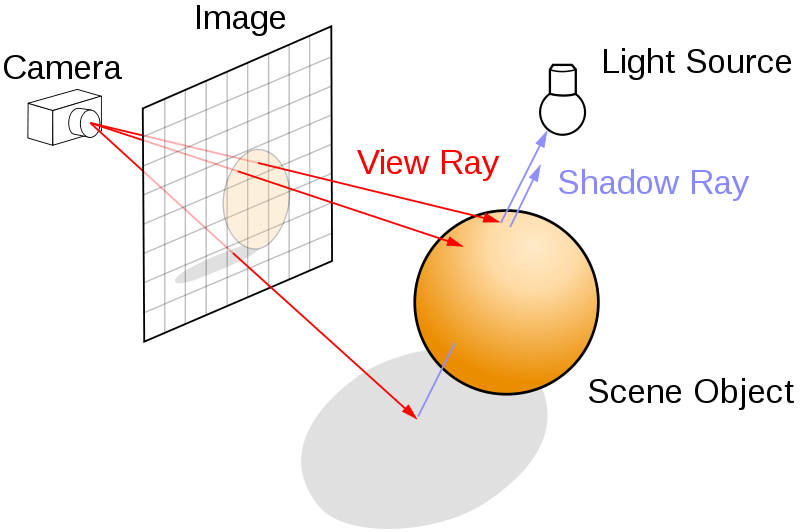
\includegraphics[scale=0.4]{res/ray_tracing.png}
\end{figure}

选定视点位置及一观察屏,从视点到屏上各点发出光线, 与空间中物体求交.
在交点处根据局部光照模型计算颜色,再递归的计算反射、透射光颜色,混合后显示在屏上.

此程序使用的局部光照模型为Phong模型,其主要公式为\cite{phong}:

\[  I_p = k_ai_a + \sum_{m\in lights} (k_d ( \overrightarrow{L_m} \cdot \overrightarrow{N} i_{m, d} + k_s(\overrightarrow{R_m}\cdot
  \overrightarrow{V})^{\alpha} i_{m, s}))  \]

其中$ k_s, k_d, k_a, \alpha$分别为物体表面该点处的高光系数,漫反射系数,环境光系数,亮度.
$ \overrightarrow{L_m}$为该点指向光源的向量, $ \overrightarrow{N}$为表面法向,
$ \overrightarrow{R_m}$为光源指向该点的光线经理想反射后的指向,
$ \overrightarrow{V}$为视点到表面交点处的向量. 实现见\verb|Space::trace()|

\subsection{全局光照模型}

程序还支持了基于Path Tracing\footnote{\url{http://en.wikipedia.org/wiki/Path_tracing}}
的全局光照模型,其渲染方程如下:

\[ L(x \rightarrow v) = L_e(x \rightarrow v)
+ \int_{\Omega}L(\Phi \rightarrow x) F_s(x, \Phi \rightarrow v)\cos \theta_{\Phi} d \Omega\]

其中, $ L(a\rightarrow b)$表示从$ b$处观察$ a$处所得结果,$ L_e$为物体自身发光亮度,$ F_s(x, \Phi \rightarrow v)$为
物体表面BRDF函数.

采用Monte Carlo Path Tracing\cite{montecarlo}对此方程进行逼近,其方法是:
在每次光线与物体的相交后, 由交点处处随机向其他方向发射多条光线, 递归求解后取平均值作为此点颜色.
随机时依据表面材质的不同选取不同的概率分布:
对于漫反射,遵循空间均匀分布,实现中, 在半球面中随机采样.
对于反射,分布近似一个尖峰函数,仅在反射方向上概率非0.
对于透射,依照Fresnel方程\cite{fresnel}计算透射比与反射比,随机选择一者进行递归.
具体实现见\verb|Space::global_trace()|.

Monte Carlo Path Tracing需要大量的采样才能够得到较好效果,因而其效率较低,
一张质量较好的图需要二十分钟渲染. 但它得到的图像更真实,如\figref{pt_diffuse}, \figref{pt_refl}, \figref{pt_transm}.

\subsection{几何对象表示及计算}
程序支持了平面、球、三角面片、包围盒四类基本几何物体,
物体都需要各自拥有与光线求交的方法.

\begin{description}
  \item[光线]光线是一条射线,包含一个起始点及方向. 见\verb|include/geometry/ray.hh|
  \item[无穷平面]
    为了计算方便,使用平面法向及平面到原点的距离作为确定平面的方式.
    平面与光线求交时,首先通过光线指向判断是否相交,再通过
    光线在平面法向方向的投影长度计算交点.见\verb|include/geometry/infplane.hh, renderable/plane.cc|

  \item[球]球由球心及半径唯一确定.球与光线求交时,
    利用球心到它在光线所在直线上的投影的距离判断是否相交,在根据投影位置及勾股定理计算交点.
    求交时要考虑光线起始点在球内部的情形,以供计算相对折射率.见\verb|include/geometry/sphere.hh, renderable/sphere.cc|

  \item[三角面片]三角面片用三个顶点坐标存储.
    为了性能,与光线的求交参考了\cite{triangle, triangle_code}的算法及实现,其基本思想是求解满足
    方程
    \[  \overrightarrow{Orig} + t  \overrightarrow{Dir} = x \overrightarrow{v_1} + y  \overrightarrow{v_2} + (1 - x -
      y)\overrightarrow{v_3}, t > 0, x, y \in (0, 1), x + y \le 1\]
    的$ (t, x, y)$, 在求交时同时能得到交点的重心坐标\footnote{\url{https://en.wikipedia.org/wiki/Barycentric\_coordinate\_system}}
    ,便于之后进行法向插值.见\verb|include/renderable/face.hh, renderable/face.cc|

  \item[轴平行包围盒]
    轴平行包围盒(Axis Align Bounding Box)用最小坐标与最大坐标两个向量存储.
    为了效率,包围盒与光线求交部分参考了\cite{aabb}的算法.
    其思想是对每个面逐一计算交点位置, 再更新最近交点.见\verb|geometry/aabb.hh|
\end{description}


\subsection{视图模型}
一个视图应包括视点及矩形屏幕,且应使视点在屏幕的中轴线上.
视图类\verb|View|存储了视点坐标,屏幕中心坐标,屏幕尺寸,屏幕边缘的两个方向向量,
并保证视点到屏幕中心的连线与屏幕边沿指向垂直.
这样可以方便的进行视图旋转,视图平移,缩放等导航操作.见\verb|include/view.hh, view.cc|

\subsection{KD树}
KD树是一种空间划分树,本用于在K维空间中快速查找区间内的点, 可利用它在光线追踪中对物体及其包围盒进行索引.
原理是,另树中每个节点对应一个包围盒,选取一个恰当的轴平行平面将包围盒一分为二, 作为两个子节点,
递归下去直至深度太大或节点内物体太少, 叶节点不仅存储包围盒, 也维护盒中物体.
注意与切分面相交的物体在左右节点中都应维护.

\subsubsection{建树}
传统的KD树中,按照使切分面两边点的个数尽量接近的原则选取切分面,其理由是假设了各个点被查询的概率均等.
而在光线追踪中,一般采用面积启发式(SAH-based)的切分面选取方式\cite{kdtree},选取切分面使得
\[ H = S_l N_l + S_r N_r \]
最大化,其中$ S_l, S_r$为左右包围盒的表面积, $ N_l, N_r$为左右包围盒管理的物体个数.
这样的建树可以使KD树在查询时效率更高.

对于启发式的建树算法, 若逐一枚举切分平面,计算包含物体个数,
需要$ O(n^2)$复杂度($n$为物体个数),程序实现了\cite{kdtree}中提供的$ O(n \log^2 n)$算法.
其优化方法是: 在每一维度上, 将各物体按坐标大小顺次选做切分平面的坐标,
因而可增量的计算平面两边包含物体的个数.实现见\verb|KDTree::build|.

对于含有20W面片的龙模型\footnote{models/fixed.perfect.dragon.100K.0.07.obj},
采用不同方法单线程建树的用时及在几个固定视角的渲染耗时如下(单位: 秒):

\begin{table}[H]
  \begin{threeparttable}
    \begin{tabular}{c|c|c|c|c|c|c}
      \shline
      & 建树 & 视角1 & 视角2 & 视角3 & 视角4 & 视角5 \\ \hline
      均分建树(终止条件:100层,15个)  & 0.6  & 1.93  & 2.51  & 3.26  & 4.38  & 5.89  \\ \hline
      SAH建树(终止条件:100层,20个) & 5.41 & 0.29  & 0.37  & 0.45  & 0.59  & 0.78    \\ \hline
      SAH建树(终止条件:100层,15个) & 7.82 & 0.24  & 0.33  & 0.41  & 0.52  & 0.68    \\ \shline
    \end{tabular}
    \begin{tablenotes}
      \footnotesize
    \item 注: 1.建树时,以树深度及当前节点所管理的物体个数作为建树终止的判定条件.
    \item 2.此实验的视角1为\verb|main.cc|中\verb|test_kdtree()|提供的视角,其余视角由视角1 zoom in依次得到.
    \item 3.可在\verb|lib/kdtree.cc|中通过注释\verb|KDTree::build()|函数中相应代码可切换两种建树算法.
    \end{tablenotes}
  \end{threeparttable}
\end{table}

由表可见SAH建树的查询效率有很大提高,但建树缓慢.
建树效率与渲染效率之间存在trade-off,可以通过改变终止条件来调整.

另外,不使用KD树时,视角1渲染时间约为800s.
(不使用KD树时, 各像素所需时间大致相同,可由部分渲染时间估算总时间).

\subsubsection{求交}
光线KD树中物体求交的基本方法是,递归寻找两子树中最近\underline{物体}(而不是叶子节点的包围盒)
的交点,取较近者为结果返回.

实现时,在每个节点处保存了两子节点的切分平面,
这样可以预先判断出首先与光线相交的包围盒,
若光线与此包围盒内物体相交, 则不用考虑另一包围盒, 提高了效率.
使用此方法应注意,若光线与较近包围盒所管理的物体相交,应确认与最近物体的\underline{交点在此包围盒内}.
因为若不包含,则光线首先打到的物体可能并不是此物体,而是第二个包围盒管理的物体.

\subsection{纹理}
一种纹理相当于一个二维坐标到表面属性的映射.
程序中的``表面属性''除包括Phong模型参数外,还包括了用于折射判定的透明度,以及全局光照模型需要使用的发光强度.
见\verb|include/material/surface.hh|.
程序实现了均匀纹理、网格纹理、图片纹理三类纹理,并可通过继承\verb|Texture|类进行扩展.

对于一个物体,由其自己管理三维坐标到二维坐标的映射.
对于平面,采用平面上的二维欧式坐标. 球体采用其极坐标.
网格未支持二维纹理,仅可以使用均匀纹理.

\subsection{法向插值}
\label{sec:smooth}
法向插值可以使三角网格表面更光滑,只需找到一个面片上的连续函数,就可以得到较好的效果.
此程序采用了线性插值.

在读入网格数据后,令各顶点法向为其相邻各面法向的平均值.
在面片与光线求交后,根据交点的重心坐标及面片各顶点的法向,即可插值出交点处法向.
效果见\figref{smooth}, \figref{simplify}.

\subsection{抗锯齿}
\begin{enumerate}
  \item 使用Beer-Lambert定律\cite{beer},使得光线亮度按传播距离指数衰减,可以有效消除远处纹理密集处的畸形.
    见\figref{first}与\figref{beer}的对比.

  \item 使用全屏抗锯齿(FSAA),对图片整体应用卷积盒$\begin{bmatrix}1 & 2 & 1\\2 & 4 & 2\\1 & 2 & 1\end{bmatrix} $,
    消除直线锯齿的同时使图片模糊,影响视觉效果.

  \item 对每一像素,计算其与周围像素距离平方之和,若小于某一阈值则应用如上卷积盒,略有效果. 见\verb|CVRender::antialias()|
\end{enumerate}

\subsection{Phong模型中的软阴影}
\label{sec:soft}
对场景中每一点光源,将其替换为点周围的多个密集点光源以模拟面光源的效果,
即可实现软阴影.效果如\figref{soft}所示, 比起Path Tracing的软阴影的话还是十分不真实. 实现见\verb|Space::add_light()|.

\subsection{景深}
程序中景深\footnote{\url{http://en.wikipedia.org/wiki/Depth\_of\_field}}
的实现方法为,以焦平面作为屏幕,取焦平面与视点之间某处建一感光器平面.
对视点到焦平面的每条光线,在它与感光器平面的交点周围随机采多个样本点,以这些样本点为观察点向
屏幕同一位置发射光线并执行光线追踪,以各样本点颜色的平均值作为最终颜色.
这样就可以使得焦平面上物体清晰,而其余位置模糊.

\verb|main.cc|中的\verb|dof_ball_scene()|生成一个演示景深的场景,场景中
可通过键盘控制焦平面位置,详见\tabref{navigate}. demo目录中有景深的演示视频.

随机取点会造成焦平面以外有无规律噪点,在生成视频后会比较明显,
因而对输出图像统一做了高斯模糊,使噪点不太明显.

\subsection{小量处理}
在如下情形需要特别注意实数运算中的误差.
\begin{enumerate}
  \item 反射折射时的交点判定

    考虑光线斜射平面的情形,若由于误差, 交点落在了平面异侧,则反射光会再次打到平面,
    若落在了平面同侧,则透射光会再次打到平面.因而计算反射光线时,
    应将其起始点回退EPS,计算透射光线时,应将其起始点前进EPS.

  \item 平行判定

    判定直线与面片或平面是否平行时,利用直线与法线点乘的绝对值$<$EPS判定,
    否则可能导致交点坐标过大, 使其他计算溢出.

  \item KD树

    建树时,对于物体与包围盒相交的判定应略微宽松,与包围盒距离$<$EPS的物体都应归入包围盒管理,
    查询时对光线与面片求交也可判的宽松一些,否则渲染的图片中容易出现黑点.

    对面片求包围盒时应注意最小值应减去EPS,最大值应加上EPS,
    否则可能出现0体积包围盒,影响算法实现.
\end{enumerate}

\subsection{网格简化}
网格的坍缩简化算法参考\cite{mesh}实现.
基本思路是,对每对顶点估算出简化代价,每次选取代价最小的顶点对执行简化操作,
操作后更新相关的代价值.

由于算法具有优先队列结构,因此使用了\verb|std::priority_queue|进行堆加速.
但由于需要执行堆元素修改操作,但STL库不支持, 因而对堆结构进行了如下处理:

对每个顶点,维护它相邻顶点中最适合坍缩的一个顶点指针.
堆元素存储一顶点指针, 它与相应邻点的坍缩代价,以及一时间戳.
堆元素按照坍缩代价保持堆性质,坍缩一对顶点后更新了附近顶点的最优代价,就将新的值打上新的时间戳插入堆中,
而取堆顶元素时,若从时间戳发现其不是最新就抛弃.
这样就可以替代修改操作.见\verb|include/mesh_simplifier.hh, mesh_simplifier.cc|

对于20万面片的龙模型\footnote{models/fixed.perfect.dragon.100K.0.07.obj},
简化掉80\%的面片需要2.37s, 而不用堆加速时需要55s.效果见\figref{simplify}及simplified目录中的图片.

\subsection{多线程}
\begin{enumerate}
  \item 对生成图片中每个像素,显然其计算相互独立,使用openmp及C++11的\verb|std::thread|两种方式对其进行多线程优化,
    效果差不多.见\verb|CVViewer::render_all()|.

  \item 建树时,两子树的创建可以并行执行.
    测试表明对根节点的两子节点并行建树有效,而对深层节点并行建树得不偿失.
    另外,$O(\log^2 n)$的建树中有一步需对各物体每一维度上的坐标排序,这是效率的瓶颈所在.
    不同维度的排序可以并行执行,经测试也只对根节点比较有效.
    这两处并行都使用C++11的\verb|std::future|实现,效率提升了约30\%.

  \item 网格简化中,对各节点代价的更新可以并行完成,效率略有提高.
\end{enumerate}

% File: proj.tex
% Date: Thu Jun 20 01:25:12 2013 +0800
% Author: Yuxin Wu <ppwwyyxxc@gmail.com>

\section{项目设计说明}

% File: diary.tex
% Date: Wed Jun 17 22:24:38 2015 +0800
% Author: Yuxin Wu <ppwwyyxxc@gmail.com>
\section{过程记录}
本项目的详细开发记录可以通过git查看. 项目托管在github\footnote{\url{https://github.com/ppwwyyxx/Ray-Tracing-Engine}}
及计算机系git9\footnote{\url{http://git.net9.org/ppwwyyxx/ray}}上,并于2013年6月24日开源.以下是一些重要记录.

以下图片中, 除最后两张效果图外, 均以800x800尺寸渲染, PDF中保留了原始尺寸的图片.
计时的机器CPU为8核 i7-3770 3.40GHz.

\begin{enumerate}
  \item
    首次出现正常的图片. 用了一个$ x-y$平面上的无限大平面及一个点光源。
    此时仅仅参考\cite{phong}考虑了基本Phong模型中的漫反射与环境光,已经可以看到左下部分亮度较高,符合预期。

    另外,远处的黑白纹理误差较大,不知是不可改进的浮点误差还是我的处理有误。
    \begin{figure}[H]
      \centering
      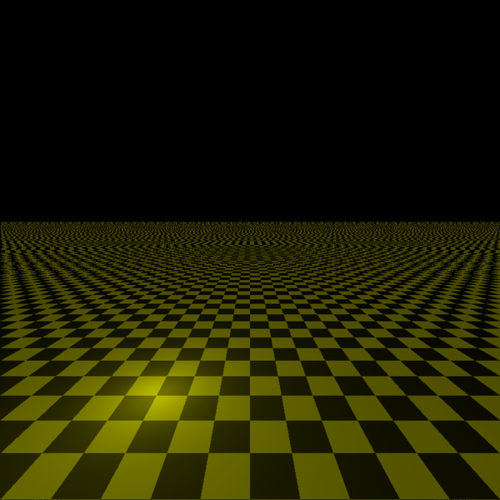
\includegraphics[scale=0.4]{img/first_pic.png}
      \caption{\label{fig:first}}
    \end{figure}

  \item
    依照Beer-Lambert定律\cite{beer}对光线能量进行了按距离的减弱:
    \[ E = E_0 e^{distance * density}\]
    使得远处的纹理更自然.
    \begin{figure}[H]
      \centering
      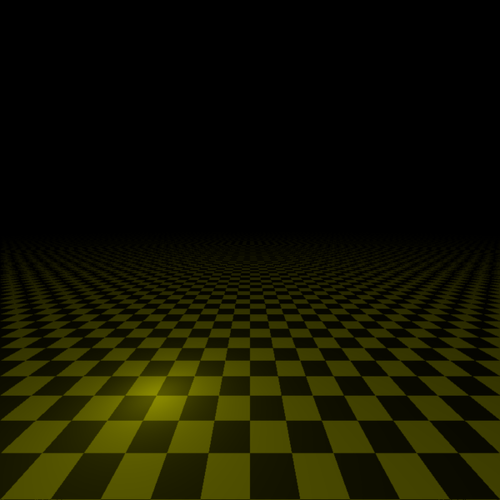
\includegraphics[scale=0.4]{img/plane_with_beer.png}
      \caption{Beer-Lambert定律效果图\label{fig:beer}}
    \end{figure}

  \item

    考虑了Phong模型中的高光,并对$ x-y$平面和$ y-z$平面加入了反射系数,有了互相反射的效果,并且
    左下部分能够看到高光.
    \begin{figure}[H]
      \centering
      
\includegraphics[scale=0.4]{img/specular.png}
      \caption*{\label{fig:specular}}
    \end{figure}

  \item

    使用球模型,可以看到明显的高光效果。同时由于球面\verb|specular|参数高,使得球下部反射了平面。
    \begin{figure}[H]
      \centering
      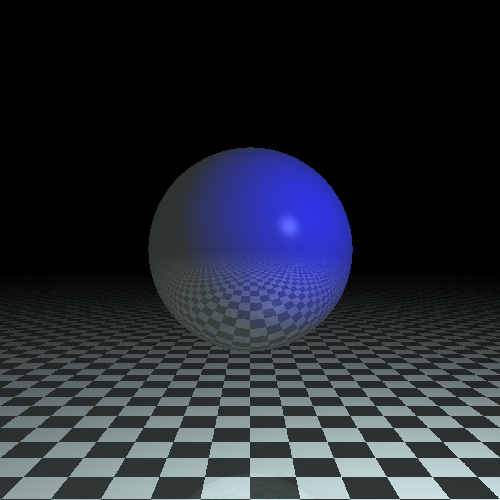
\includegraphics[scale=0.4]{img/ball.png}
      \caption*{\label{fig:ball}}
    \end{figure}

  \item
    对于找到的交点,判断它与光源之间是否被挡住,若被挡住就不计算漫反射和高光. 这样实现了阴影效果.
    \begin{figure}[H]
      \centering
      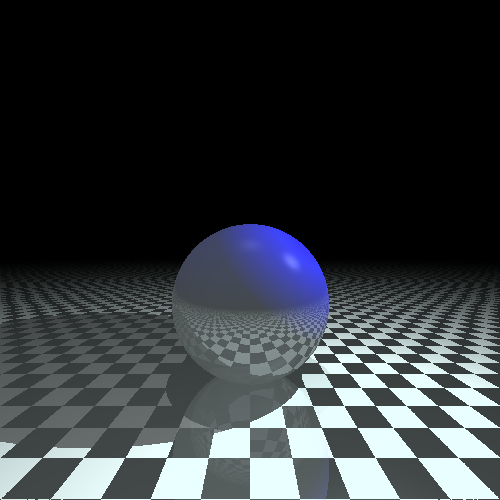
\includegraphics[scale=0.4]{img/shadow.png}
      \caption*{\label{fig:shadow}}
    \end{figure}

  \item 对根据视点及对象生成视图(View)的方案进行修改,以支持视图的旋转,缩放.并利用opencv的key event实现了gui的旋转,缩放控制.
    \begin{figure}[H]
      \centering
      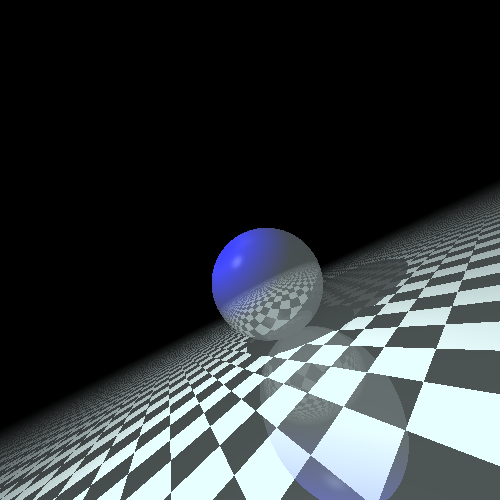
\includegraphics[scale=0.4]{img/rotate.png}
      \caption*{\label{fig:rotate}}
    \end{figure}

  \item 加入了透射功能,依照预定义的介质密度及折射定律计算出射光方向.
    \begin{figure}[H]
      \centering
      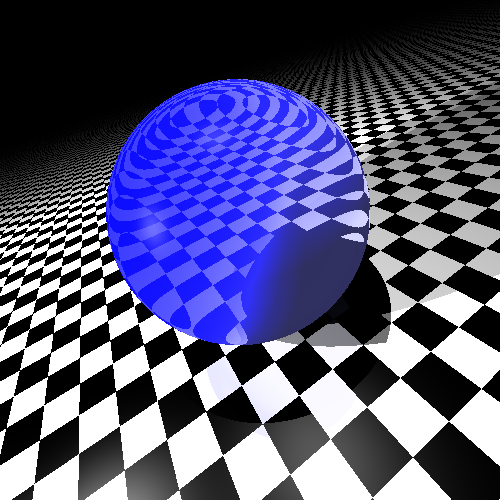
\includegraphics[scale=0.4]{img/transmission.png}
      \caption*{\label{fig:transmission}}
    \end{figure}

  \item 实现了三角面片的渲染,在求交时计算齐次重心坐标,为网格中的法向插值做准备.
    \begin{figure}[H]
      \centering
      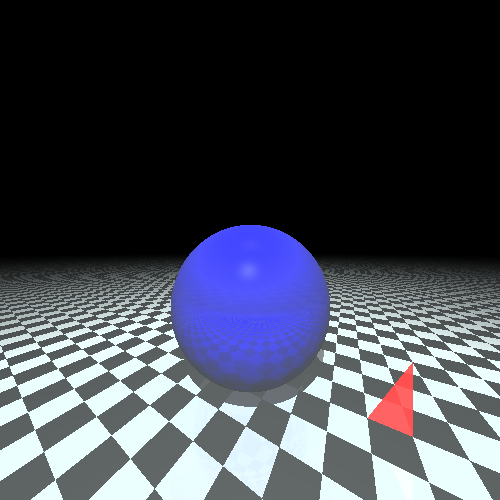
\includegraphics[scale=0.4]{img/face.png}
      \caption*{\label{fig:face}}
    \end{figure}

  \item 实现了obj格式读取及基本的渲染,绘制出了一个红色小人.
    \begin{figure}[H]
      \centering
      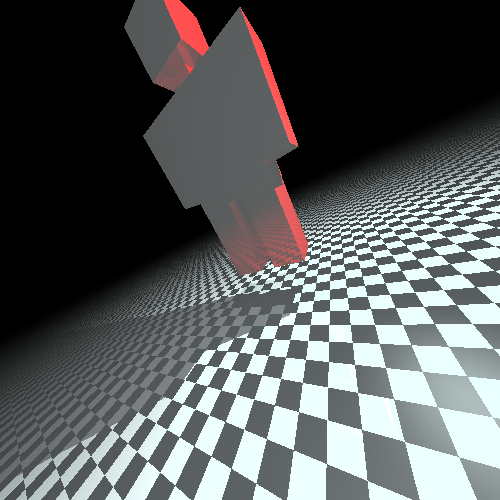
\includegraphics[scale=0.4]{img/human.png}
      \caption*{\label{fig:human}}
    \end{figure}

  \item 实现了KDTree, 可以开始渲染更大的obj.
    \begin{figure}[H]
      \centering
      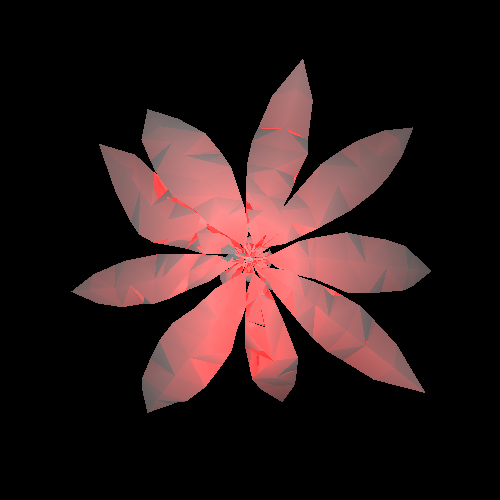
\includegraphics[scale=0.4]{img/flower.png}
      \caption*{\label{fig:flower}}
    \end{figure}

  \item 按照\cite{kdtree}优化了KDTree的实现之后发现如下左图所示bug, 调试很久后发现两个原因.
    一是建树时选取候选切割平面未偏移\verb|EPS|, 二是包围盒求交存在小bug,少了一个绝对值运算.
    其中第二个bug还严重影响了速度,修复后的KDTree相比不用KDTree有了上千倍的速度提升.
    \begin{figure}[H]
      \centering
      \begin{minipage}[b]{0.46\linewidth}
        \centering
        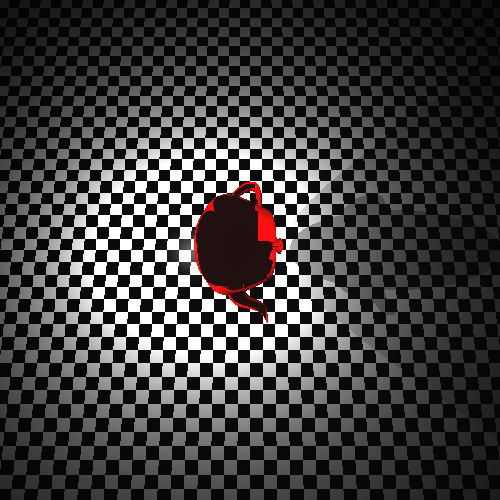
\includegraphics[width=\textwidth]{img/bug_teapot.png}
      \end{minipage}
      \begin{minipage}[b]{0.46\linewidth}
        \centering
        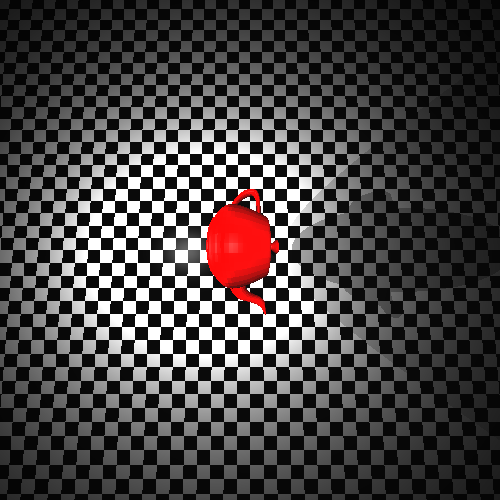
\includegraphics[width=\textwidth]{img/fixed_teapot.png}
      \end{minipage}
      \caption*{\label{fig:kdtree_bug}}
    \end{figure}

  \item 实现了法向量插值,详见\secref{smooth}. 插值前后的效果如下所示:
    \begin{figure}[H]
      \begin{minipage}[b]{0.46\linewidth}
        \centering
        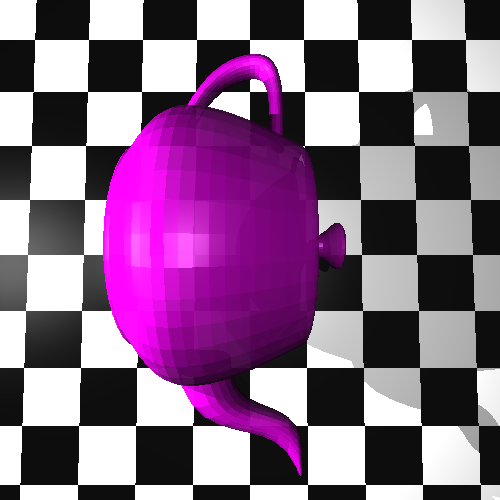
\includegraphics[width=\textwidth]{img/rough.png}
      \end{minipage}
      \begin{minipage}[b]{0.46\linewidth}
        \centering
        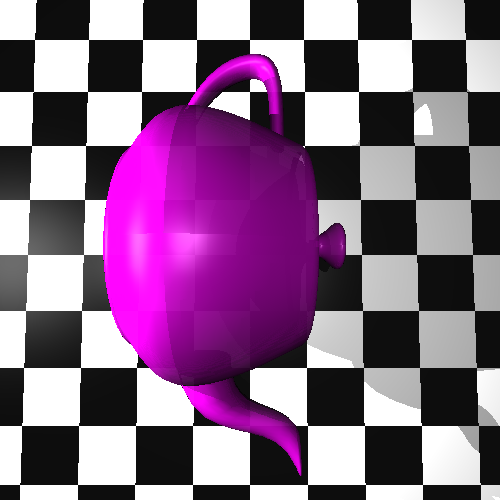
\includegraphics[width=\textwidth]{img/smooth.png}
      \end{minipage}
      \caption{插值的茶壶\label{fig:smooth}}
    \end{figure}

  \item 将KDTree扩展到了整个空间.
    设计方法是将所有的有限大物体合成为一个``KDTree''物体,保留无限大物体,再在
    空间中进行渲染.下图是一个20W面片的龙加上1万个球组成的场景,渲染此图只需1.4s.
    \begin{figure}[H]
      \centering
      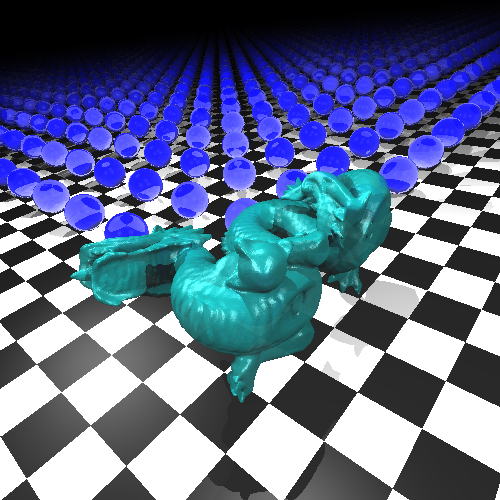
\includegraphics[scale=0.4]{img/dragonball.png}
      \caption*{\label{fig:dragonball}}
    \end{figure}

  \item 加入了图片纹理,设置在平面上.(图中亮斑为点光源所致)
    \begin{figure}[H]
      \centering
      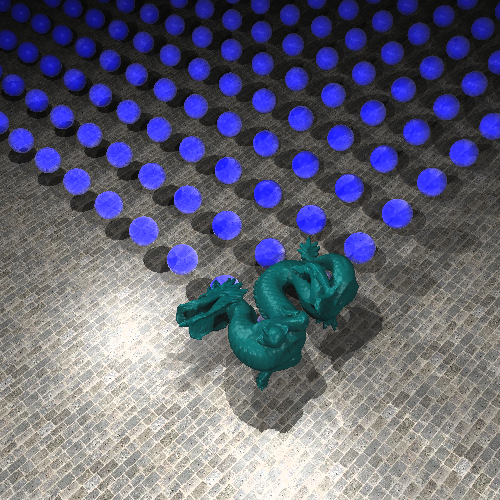
\includegraphics[scale=0.4]{img/pic_texture.png}
      \caption*{\label{fig:texture}}
    \end{figure}

  \item 加入了软阴影效果,详见\secref{soft}.将每个点光源变为20个密集点光源可使左图场景渲染出右图效果.
    左图渲染时间为0.15s, 右图为1.06s
    \begin{figure}[H]
      \begin{minipage}[b]{0.46\linewidth}
        \centering
        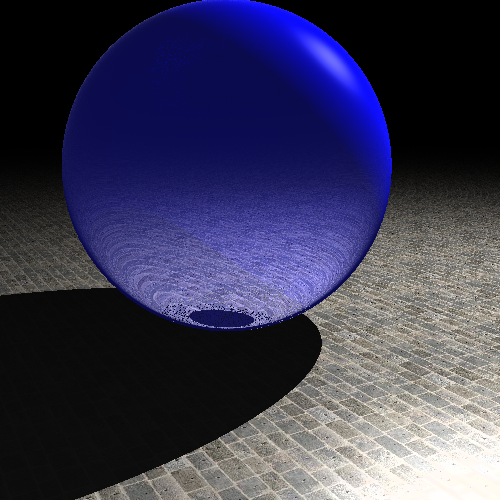
\includegraphics[width=\textwidth]{img/no_soft.png}
      \end{minipage}
      \begin{minipage}[b]{0.46\linewidth}
        \centering
        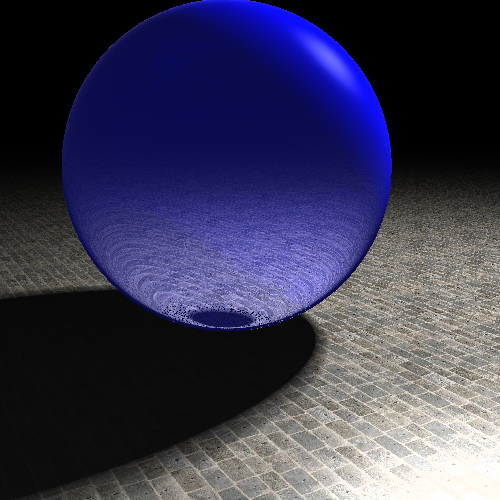
\includegraphics[width=\textwidth]{img/soft.png}
      \end{minipage}
      \caption{软阴影效果图\label{fig:soft}}
    \end{figure}

  \item 加入了抗锯齿效果,能看出变化但效果不明显. 为了图片清晰将此功能关闭.

  \item 发现球与地面接触处有密集的小斑点,调试后发现是由于球底部与平面略微重合,求交时有时会出错.
    \begin{figure}[H]
      \centering
      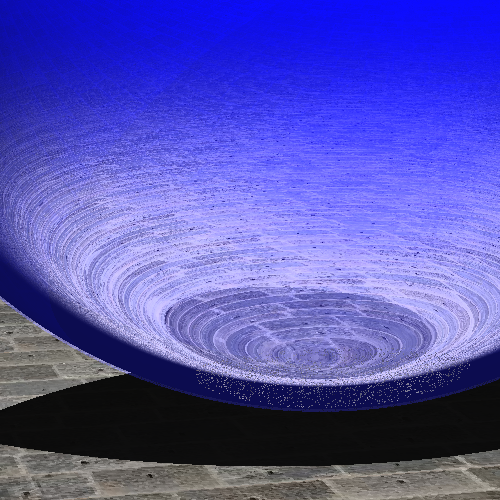
\includegraphics[scale=0.4]{img/smallpoint.png}
    \end{figure}

  \item 加入了景深效果,在感光器处随机取了20个伪视点,效率也相应降低了20倍,效果如图所示.
    \begin{figure}[H]
      \centering
      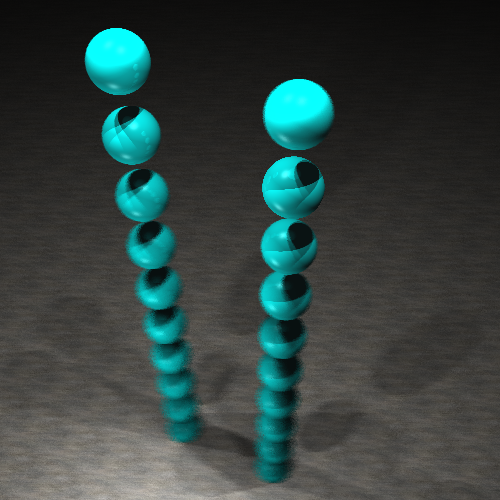
\includegraphics[scale=0.4]{img/dof.png}
      \caption*{\label{fig:dof}}
    \end{figure}

  \item 由于\verb|std::shared_ptr<T>|的默认构造函数会对引用计数和指针对象进行两次内存分配,效率不够高.
    大量换用\verb|std::make_share<T>|后光线追踪时间缩短了40\%.

  \item 利用C++11中的\verb|std::future|实现了KDTree树构建的多线程,建树提速30\%.

  \item 实现了网格简化,并利用堆加速. 对20万面片龙,效果如下.
    \begin{figure}[H]
      \begin{minipage}[b]{0.46\linewidth}
        \centering
        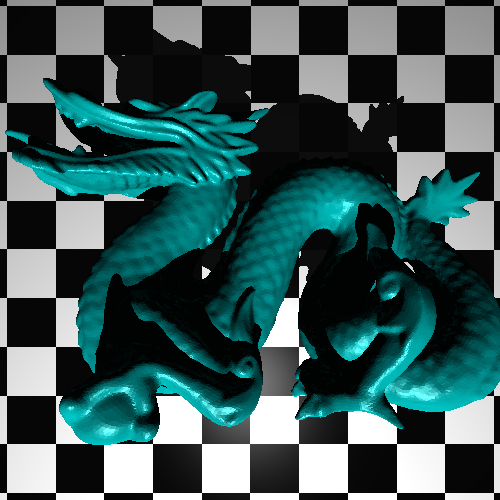
\includegraphics[width=\textwidth]{img/unsimplified_nosmooth.png}
        \caption*{未简化,无法向插值}
      \end{minipage}
      \begin{minipage}[b]{0.46\linewidth}
        \centering
        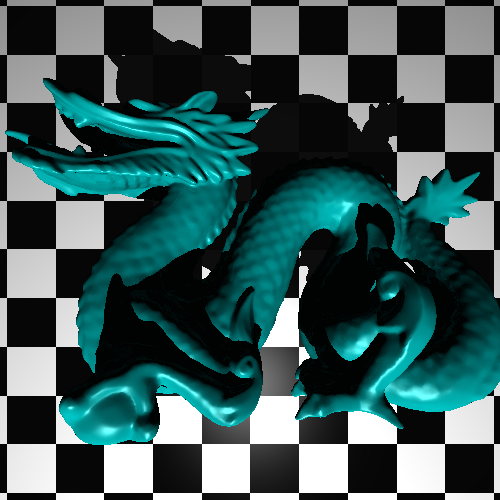
\includegraphics[width=\textwidth]{img/unsimplified_smooth.png}
        \caption*{未简化,含法向插值}
      \end{minipage}

      \begin{minipage}[b]{0.46\linewidth}
        \centering
        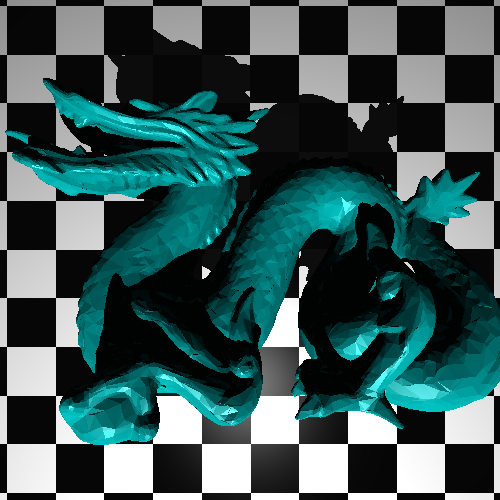
\includegraphics[width=\textwidth]{img/simplified_nosmooth.png}
        \caption*{简化至20\%, 无法向插值}
      \end{minipage}
      \begin{minipage}[b]{0.46\linewidth}
        \centering
        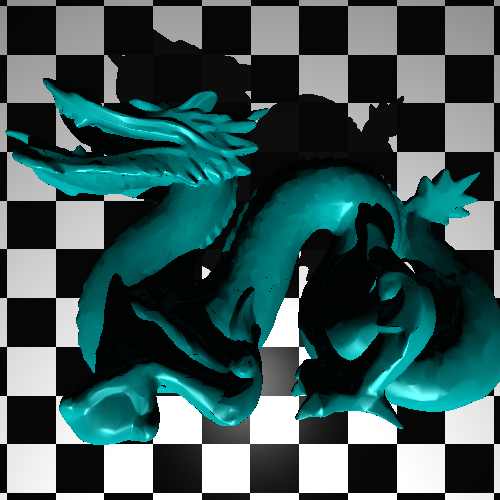
\includegraphics[width=\textwidth]{img/simplified_smooth.png}
        \caption*{简化至20\%, 含法向插值}
      \end{minipage}
      \caption{网格简化效果图\label{fig:simplify}}

    \end{figure}

  \item 发现对于某些模型,简化时会触发\verb|assert|,调试后发现是由于网格坍缩时可能会导致一个面片中三点共线从而无法正确计算出法向.
    将其修正为:若坍缩后面片三点共线,则保留原法向.

  \item 发现在调用\verb|Space::add_obj()|后,若在调用栈中将\verb|Mesh|析构,则会发生段错误.调试很久后发现是由于
    \verb|Face|类中存储了指向其宿主的指针\verb|Mesh* host|,用于获取插值及纹理信息用,此指针在\verb|Mesh|复制时未被正确更新导致
    得不到其宿主.


  \item 利用Qt4实现了一个简单的GUI,支持单个obj的预览,视点移动,网格简化.

    \begin{figure}[H]
      \centering
      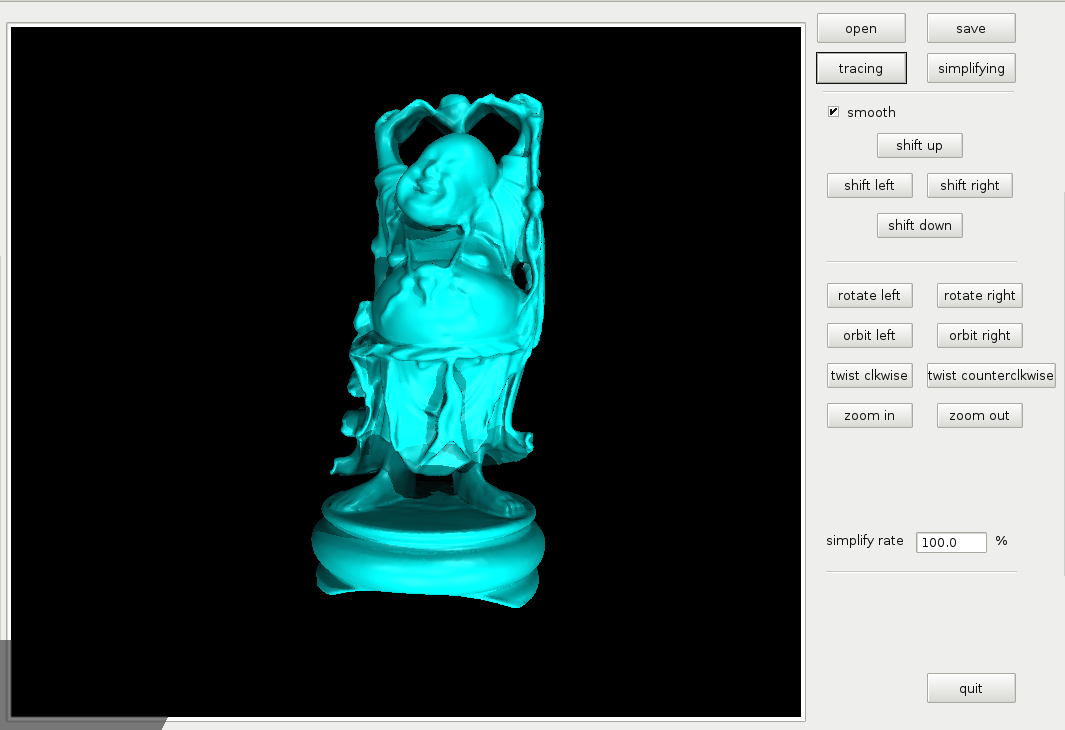
\includegraphics[scale=0.38]{img/gui.png}
      \caption{图形界面展示\label{fig:gui}}
    \end{figure}

  \item 实现了一个简易的全局光照模型,首先按照均匀分布支持了漫反射,渲染效果如下.
    可以看到颜色变化及阴影都比右图的Phong模型更自然.
    \begin{figure}[H]
      \begin{minipage}[b]{0.48\linewidth}
        \centering
        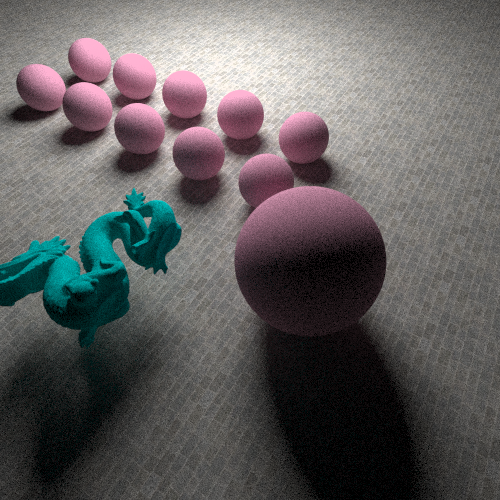
\includegraphics[width=\textwidth]{img/gllu_first.png}
      \end{minipage}
      \begin{minipage}[b]{0.48\linewidth}
        \centering
        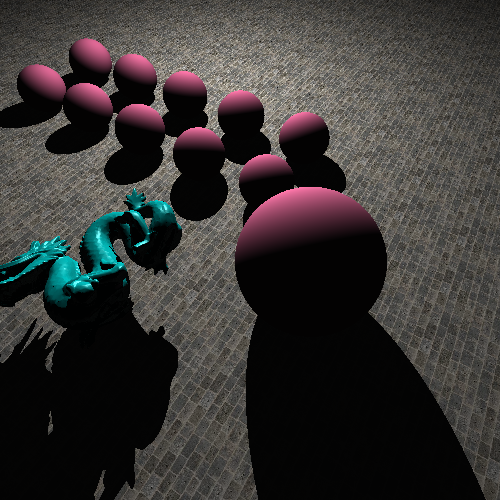
\includegraphics[width=\textwidth]{img/compare_diffuse_phong.png}
      \end{minipage}
      \caption{Path Tracing漫反射效果图(左)\label{fig:pt_diffuse}}
    \end{figure}

  \item 为全局光照模型加入了镜面反射效果,若干个镜面的球上可以看到光源的亮斑及互相的反射,如下左图.
    \begin{figure}[H]
      \begin{minipage}[b]{0.48\linewidth}
        \centering
        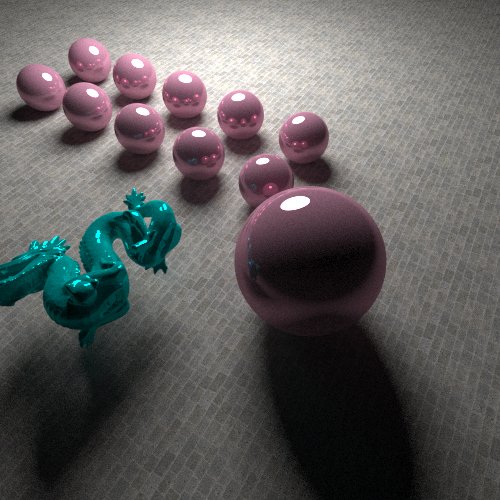
\includegraphics[width=\textwidth]{img/gllu_refl.png}
      \end{minipage}
      \begin{minipage}[b]{0.48\linewidth}
        \centering
        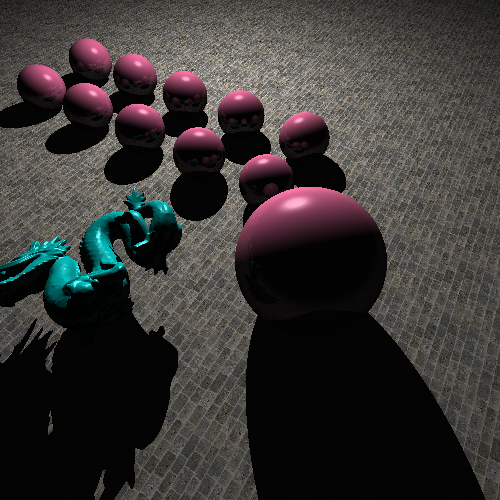
\includegraphics[width=\textwidth]{img/compare_refl_phong.png}
      \end{minipage}
      \caption{Path Tracing镜面效果图(左)\label{fig:pt_refl}}
    \end{figure}

  \item 加入了全局光照模型的折射效果,结果很逼真,可以看到球下方的caustic效果,Phong模型通常无法模拟此效果.
    \begin{figure}[H]
      \centering
      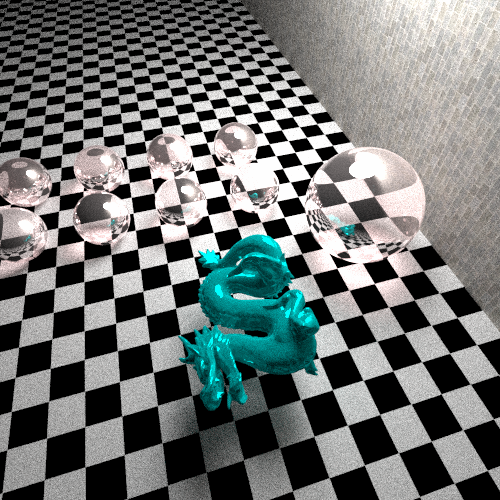
\includegraphics[scale=0.5]{img/caustic.png}
      \caption{Path Tracing透射效果图\label{fig:pt_transm}}
    \end{figure}

\end{enumerate}

\section*{两张效果图}
\begin{figure}[H]
  \centering
  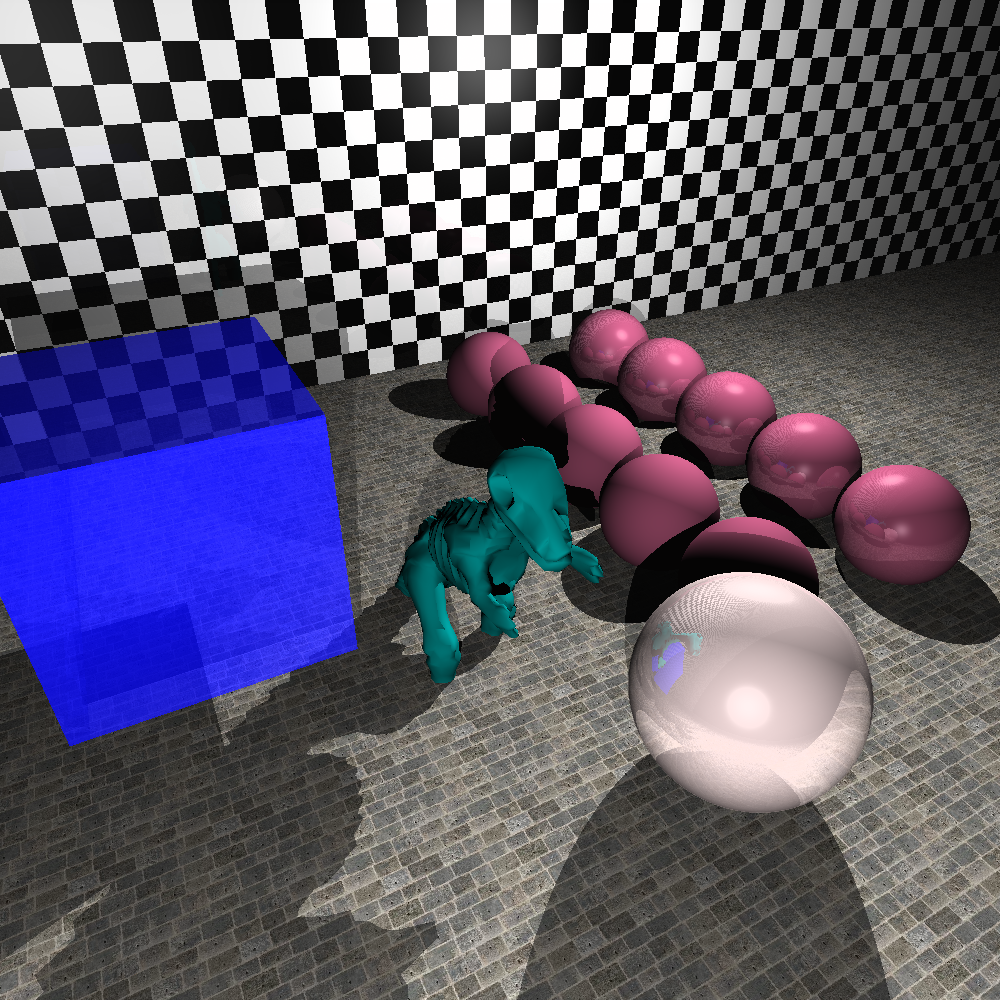
\includegraphics[width=\textwidth]{img/all_phong.png}
\end{figure}

\begin{figure}[H]
  \centering
  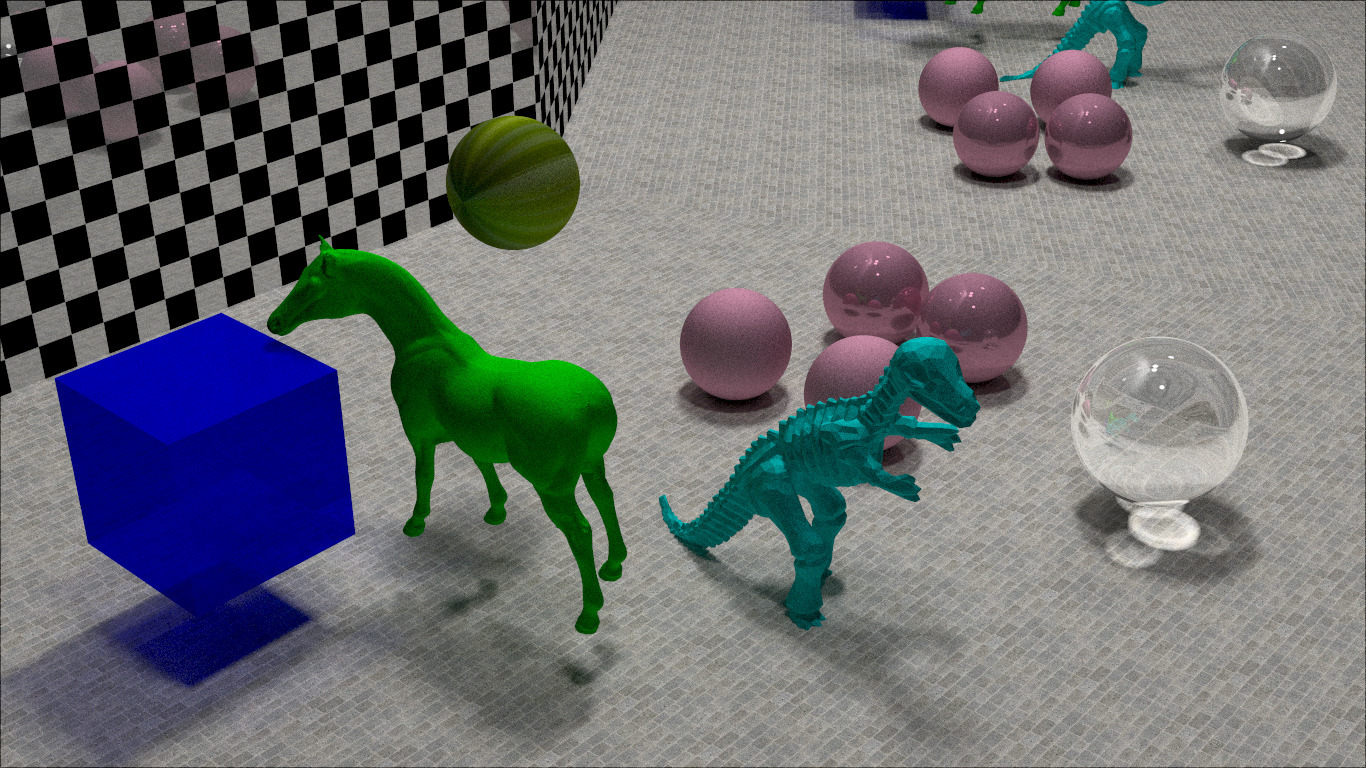
\includegraphics[width=\textwidth]{img/all_path_tracing.jpg}
\end{figure}

\printbibliography

\end{document}

